\documentclass[11pt]{article}

% Generated by tools/author/maptex.py. Do not edit; edit the map's author script
% and run it again.

\usepackage[T1]{fontenc}
\usepackage[utf8]{inputenc}
\usepackage[margin=0.85in]{geometry}
\usepackage{amsmath}
\usepackage{kpfonts}
\usepackage{tikz}
\usetikzlibrary{arrows.meta}
\usepackage{enumitem}
\usepackage{multicol}
\usepackage{xcolor}

\definecolor{maroon}{HTML}{800000}
\definecolor{inkgrey}{HTML}{4D4D4D}

% An explicit white page. Without it the page background is undefined, and a viewer
% or a converter that composites onto black renders the body text invisible.
\pagecolor{white}

\pagestyle{empty}
\setlength{\parindent}{0pt}
\setlength{\parskip}{0.6em}

\newcommand{\heading}[1]{%
  \par\medskip{\large\bfseries\color{maroon} #1}\par\smallskip}

\tikzset{
  concept/.style={rectangle, draw=inkgrey, rounded corners=2pt,
    align=center, font=\footnotesize, inner sep=3pt, fill=white, line width=0.5pt},
  edgenum/.style={circle, fill=white, draw=inkgrey, inner sep=0pt,
    minimum size=11pt, font=\scriptsize\bfseries, line width=0.4pt},
  nlabel/.style={font=\tiny\bfseries, text=inkgrey, inner sep=1pt},
  % One style for every arrow on the blank sheet. Which of the four kinds it is is
  % part of the question, so the drawing must not answer it.
  arr/.style={-, thick, inkgrey},
  % On the answer key each kind is drawn as itself, so the kinds can be checked off
  % the picture as well as read off the list. No hyphens in these names: tikz reads
  % a hyphen in a style name as an arrow-tip spec.
  kindimplies/.style={-{Latex[length=2mm]}, thick, green!45!black},
  kindfails/.style={-{Latex[length=2mm]}, thick, dashed, red!65!black},
  kindequiv/.style={{Latex[length=2mm]}-{Latex[length=2mm]}, thick, blue!60!black},
}

\begin{document}

{\LARGE\bfseries\color{maroon} Infinite series: answers}\par\medskip
{\color{inkgrey}\small Math 163 \quad\textbullet\quad Prof.\ Chowdhury}\par\bigskip

Every arrow, with the kind of relationship it is. On this copy each arrow is drawn in the style of its kind, so you can check the kinds off the picture as well as off the list.

\heading{What each box means}
\small
\begin{enumerate}[label=\textbf{\Alph*.}, leftmargin=2.2em, itemsep=1pt]
\item \textbf{Infinite Series \(\sum a_n\).} The expression \(a_1 + a_2 + a_3 + \cdots\). It has no meaning until the partial sums give it one.
\item \textbf{Partial Sums \(\{s_n\}\).} \(s_n = a_1 + \cdots + a_n\). An ordinary sequence, so everything you know about sequences applies to it.
\item \textbf{Convergent Series.} \(\sum a_n\) converges when \(\{s_n\}\) has a finite limit, and the sum is that limit.
\item \textbf{Divergent Series.} \(\sum a_n\) diverges when \(\{s_n\}\) fails to converge, whether it runs away or oscillates.
\item \textbf{Divergence Test.} If \(a_n \not\to 0\) then \(\sum a_n\) diverges. It is a test for divergence only, and it never certifies convergence.
\item \textbf{Geometric Series.} \(\sum ar^n\), which converges exactly when \(|r| < 1\), with sum \(a/(1-r)\) and partial sums \(a(1-r^n)/(1-r)\).
\item \textbf{Telescoping Series.} \(\sum (b_n - b_{n+1})\), whose partial sums collapse to \(b_1 - b_{n+1}\).
\item \textbf{\(p\)-Series \(\sum 1/n^p\).} Converges exactly when \(p > 1\). The boundary \(p = 1\) is the harmonic series, which diverges.
\item \textbf{Nonneg Series \(+\) MCT.} If \(a_n \ge 0\) the partial sums increase, so the monotone convergence theorem turns convergence into boundedness.
\item \textbf{Comparison Tests.} Direct: \(0 \le a_n \le cb_n\) eventually and \(\sum b_n\) convergent gives \(\sum a_n\) convergent. Limit: \(\lim a_n/b_n \in (0,\infty)\) gives the same behaviour for both.
\item \textbf{Integral Test.} If \(f\) is positive, continuous and eventually decreasing with \(f(n) = a_n\), then \(\sum a_n\) and \(\int_1^\infty f\) converge or diverge together.
\item \textbf{Dirichlet's Test.} If \(a_n\) decreases to \(0\) and the partial sums of \(b_n\) are bounded, then \(\sum a_n b_n\) converges. Proved by summation by parts.
\item \textbf{Absolute Convergence.} \(\sum a_n\) converges absolutely when \(\sum |a_n|\) converges. This is strictly stronger than convergence.
\item \textbf{Conditional Convergence.} \(\sum a_n\) converges conditionally when it converges and \(\sum |a_n|\) does not. The convergence rests on cancellation.
\item \textbf{Ratio and Root Tests.} With \(L = \lim |a_{n+1}/a_n|\) or \(L = \limsup |a_n|^{1/n}\): absolutely convergent if \(L < 1\), divergent if \(L > 1\), and no conclusion if \(L = 1\).
\end{enumerate}
\normalsize
\heading{Counterexamples and benchmarks}
\small
\begin{itemize}[leftmargin=1.4em, itemsep=1pt]
\item The harmonic series \(\sum 1/n\) diverges even though its terms tend to zero.
\item The alternating harmonic series \(\sum (-1)^{n+1}/n\) converges conditionally, to \(\ln 2\).
\item \(\sum \sin(n\theta)/n\) converges by Dirichlet's test and is not alternating.
\item Summation by parts is the discrete integration by parts, and it is what proves Dirichlet's test.
\item The Cauchy criterion for series: control every far enough tail at once, not one chosen tail.
\end{itemize}
\normalsize
\newpage
\vspace*{\fill}
\begin{center}
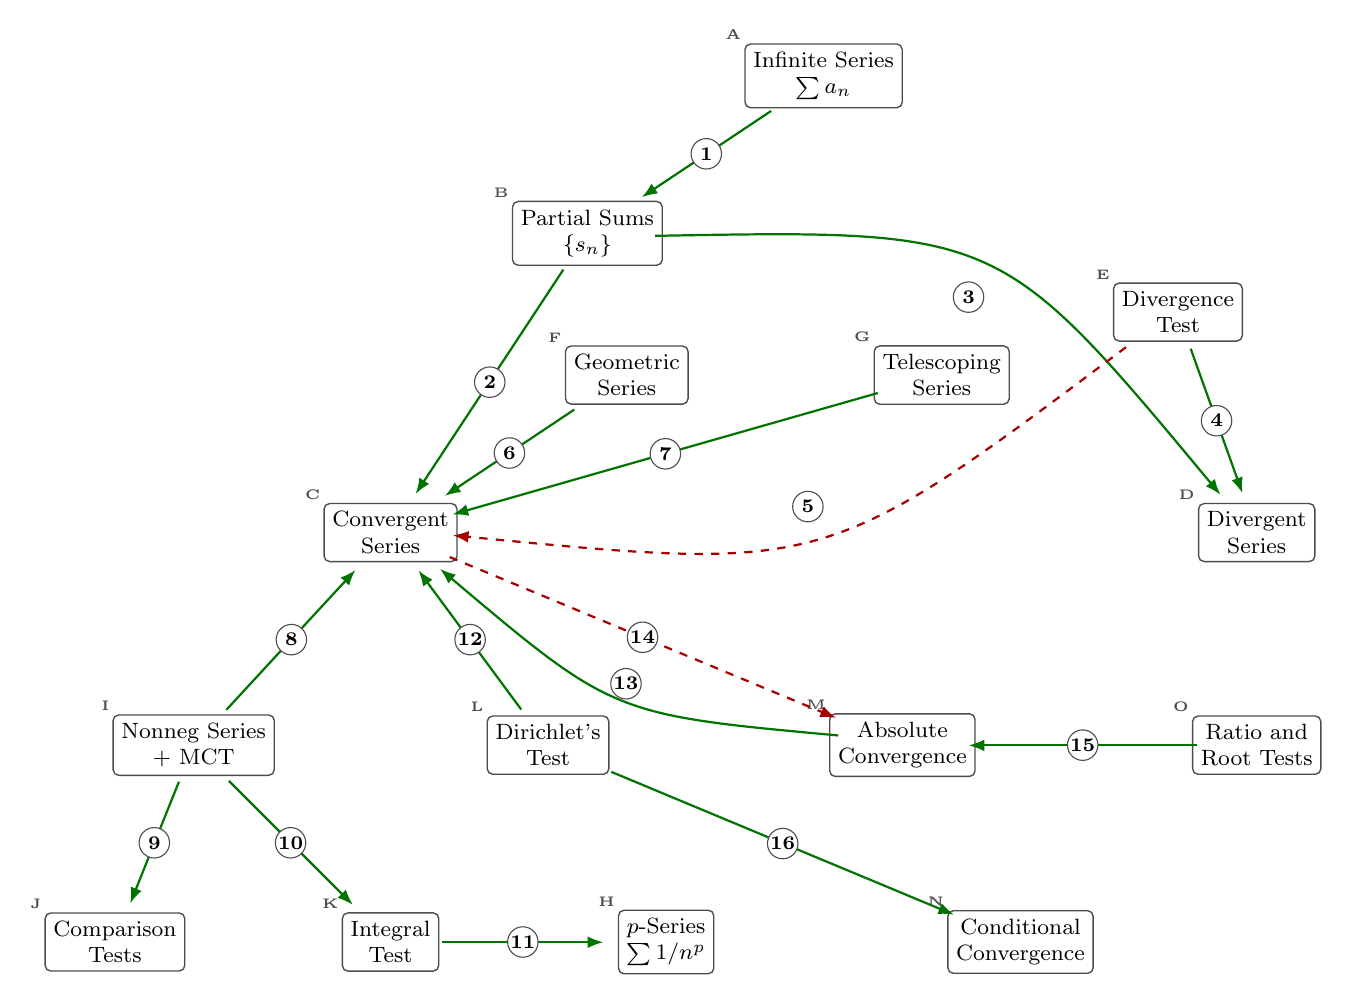
\begin{tikzpicture}[>=Latex]
  \node[concept] (A) at (1.5, 0) {Infinite Series \\ \(\sum a_n\)};
  \node[concept] (B) at (-1.5, -2) {Partial Sums \\ \(\{s_n\}\)};
  \node[concept] (C) at (-4, -5.8) {Convergent \\ Series};
  \node[concept] (D) at (7, -5.8) {Divergent \\ Series};
  \node[concept] (E) at (6, -3) {Divergence \\ Test};
  \node[concept] (F) at (-1, -3.8) {Geometric \\ Series};
  \node[concept] (G) at (3, -3.8) {Telescoping \\ Series};
  \node[concept] (H) at (-0.5, -11) {\(p\)-Series \\ \(\sum 1/n^p\)};
  \node[concept] (I) at (-6.5, -8.5) {Nonneg Series \\ \(+\) MCT};
  \node[concept] (J) at (-7.5, -11) {Comparison \\ Tests};
  \node[concept] (K) at (-4, -11) {Integral \\ Test};
  \node[concept] (L) at (-2, -8.5) {Dirichlet's \\ Test};
  \node[concept] (M) at (2.5, -8.5) {Absolute \\ Convergence};
  \node[concept] (N) at (4, -11) {Conditional \\ Convergence};
  \node[concept] (O) at (7, -8.5) {Ratio and \\ Root Tests};

  \node[nlabel, anchor=south east] at (A.north west) {A};
  \node[nlabel, anchor=south east] at (B.north west) {B};
  \node[nlabel, anchor=south east] at (C.north west) {C};
  \node[nlabel, anchor=south east] at (D.north west) {D};
  \node[nlabel, anchor=south east] at (E.north west) {E};
  \node[nlabel, anchor=south east] at (F.north west) {F};
  \node[nlabel, anchor=south east] at (G.north west) {G};
  \node[nlabel, anchor=south east] at (H.north west) {H};
  \node[nlabel, anchor=south east] at (I.north west) {I};
  \node[nlabel, anchor=south east] at (J.north west) {J};
  \node[nlabel, anchor=south east] at (K.north west) {K};
  \node[nlabel, anchor=south east] at (L.north west) {L};
  \node[nlabel, anchor=south east] at (M.north west) {M};
  \node[nlabel, anchor=south east] at (N.north west) {N};
  \node[nlabel, anchor=south east] at (O.north west) {O};

  \draw[kindimplies] (0.833, -0.446) .. controls (0.011, -0.994) .. (-0.811, -1.542);
  \draw[kindimplies] (-1.805, -2.46) .. controls (-2.744, -3.886) .. (-3.683, -5.311);
  \draw[kindimplies] (-0.641, -2.032) .. controls (3.739, -1.952) .. (6.54, -5.321);
  \draw[kindimplies] (6.162, -3.466) .. controls (6.491, -4.384) .. (6.819, -5.302);
  \draw[kindfails] (5.34, -3.446) .. controls (1.529, -6.301) .. (-3.21, -5.835);
  \draw[kindimplies] (-1.667, -4.239) .. controls (-2.489, -4.787) .. (-3.311, -5.335);
  \draw[kindimplies] (2.188, -4.028) .. controls (-0.513, -4.799) .. (-3.214, -5.571);
  \draw[kindimplies] (-6.086, -8.052) .. controls (-5.265, -7.163) .. (-4.444, -6.274);
  \draw[kindimplies] (-6.688, -8.965) .. controls (-6.997, -9.737) .. (-7.306, -10.51);
  \draw[kindimplies] (-6.053, -8.954) .. controls (-5.266, -9.741) .. (-4.478, -10.529);
  \draw[kindimplies] (-3.348, -11.003) .. controls (-2.322, -11.003) .. (-1.297, -11.003);
  \draw[kindimplies] (-2.34, -8.048) .. controls (-2.993, -7.164) .. (-3.646, -6.28);
  \draw[kindimplies] (1.687, -8.377) .. controls (-1.175, -8.115) .. (-3.372, -6.261);
  \draw[kindfails] (-3.249, -6.111) .. controls (-0.795, -7.133) .. (1.658, -8.154);
  \draw[kindimplies] (6.238, -8.503) .. controls (4.79, -8.503) .. (3.341, -8.503);
  \draw[kindimplies] (-1.197, -8.839) .. controls (0.981, -9.747) .. (3.158, -10.654);

  \node[edgenum] at (0.01, -0.99) {1};
  \node[edgenum] at (-2.74, -3.89) {2};
  \node[edgenum] at (3.34, -2.81) {3};
  \node[edgenum] at (6.49, -4.38) {4};
  \node[edgenum] at (1.30, -5.47) {5};
  \node[edgenum] at (-2.49, -4.79) {6};
  \node[edgenum] at (-0.51, -4.80) {7};
  \node[edgenum] at (-5.26, -7.16) {8};
  \node[edgenum] at (-7.00, -9.74) {9};
  \node[edgenum] at (-5.27, -9.74) {10};
  \node[edgenum] at (-2.32, -11.00) {11};
  \node[edgenum] at (-2.99, -7.16) {12};
  \node[edgenum] at (-1.01, -7.72) {13};
  \node[edgenum] at (-0.80, -7.13) {14};
  \node[edgenum] at (4.79, -8.50) {15};
  \node[edgenum] at (0.98, -9.75) {16};
\end{tikzpicture}
\end{center}
\begin{center}\small
\textcolor{green!45!black}{\textbf{---\!\!\textgreater\ gives}} \quad \textcolor{red!65!black}{\textbf{--\,--\!\!\textgreater\ fails}} \quad \textcolor{blue!60!black}{\textbf{\textless\!\!---\!\!\textgreater\ both ways}}
\end{center}
\vspace*{\fill}
\newpage
\heading{The arrows}
\small
\begin{multicols}{2}
\begin{enumerate}[label=\textbf{\arabic*.}, itemsep=0.55em, leftmargin=1.8em]
\item
  {\scriptsize\bfseries\color{maroon} gives.}\ Convergence of the series is defined to be convergence of its sequence of partial sums.
  {\scriptsize\color{inkgrey} Nothing else defines it. Every test in this chapter is a statement about the partial sums, reached without ever computing them.\par}
\item
  {\scriptsize\bfseries\color{maroon} gives.}\ If the partial sums have a finite limit then the series converges, and its sum is that limit.
  {\scriptsize\color{inkgrey} The definition read from left to right.\par}
\item
  {\scriptsize\bfseries\color{maroon} gives.}\ If the partial sums fail to converge then the series diverges, and running off to infinity is only one of the ways that happens.
  {\scriptsize\color{inkgrey} Divergence is the negation of convergence, so unbounded partial sums and oscillating ones are both covered by it.\par}
\item
  {\scriptsize\bfseries\color{maroon} gives.}\ Terms that do not tend to zero leave the partial sums unable to settle, so the series diverges.
  {\scriptsize\color{inkgrey} The difference \(s_n - s_{n-1}\) is \(a_n\). If \(s_n\) had a limit, that difference would have to tend to zero.\par}
\item
  {\scriptsize\bfseries\color{maroon} fails.}\ Terms tending to zero is necessary for convergence and not sufficient for it, and the harmonic series is the witness.
  {\scriptsize\color{inkgrey} \(1/n \to 0\) while \(\sum 1/n\) diverges, by Nicole Oresme's grouping of the terms into blocks each contributing at least \(1/2\).\par}
\item
  {\scriptsize\bfseries\color{maroon} gives.}\ A geometric series converges exactly when its ratio has modulus below one, and then the closed form for the partial sums gives the sum.
  {\scriptsize\color{inkgrey} One of the two series here whose partial sums you can write down, which is why the comparison tests are run against it.\par}
\item
  {\scriptsize\bfseries\color{maroon} gives.}\ In a telescoping series consecutive terms cancel, so the partial sums collapse and converge exactly when \(b_n\) does.
  {\scriptsize\color{inkgrey} The other series whose partial sums you can write down. The sum is \(b_1\) minus the limit of \(b_n\).\par}
\item
  {\scriptsize\bfseries\color{maroon} gives.}\ For a series of nonnegative terms the partial sums increase, so the series converges exactly when they are bounded above.
  {\scriptsize\color{inkgrey} This is what every test for a nonnegative series is really using. Boundedness has replaced the limit, and a bound is something you can find without knowing the sum.\par}
\item
  {\scriptsize\bfseries\color{maroon} gives.}\ Bounding a nonnegative series term by term against a series you already know bounds its partial sums.
  {\scriptsize\color{inkgrey} Direct comparison bounds the partial sums; limit comparison compares growth rates instead and reaches the same conclusion for both series.\par}
\item
  {\scriptsize\bfseries\color{maroon} gives.}\ Comparing a decreasing positive term with the area under the matching function bounds the partial sums by an improper integral.
  {\scriptsize\color{inkgrey} The rectangles drawn on either side of the graph give the two inequalities, and both of them need \(f\) positive, continuous and eventually decreasing.\par}
\item
  {\scriptsize\bfseries\color{maroon} gives.}\ Running the integral test on \(1/x^p\) puts the threshold for the \(p\)-series at \(p = 1\).
  {\scriptsize\color{inkgrey} \(\int_1^\infty x^{-p}\,dx\) is finite exactly when \(p > 1\), and \(p = 1\) is the harmonic series on the wrong side of the line.\par}
\item
  {\scriptsize\bfseries\color{maroon} gives.}\ A sequence decreasing to zero paired with bounded partial sums gives a convergent series, and the alternating series test is the case where the second factor is \((-1)^n\).
  {\scriptsize\color{inkgrey} The proof is summation by parts, which is the discrete version of integration by parts. For a case that is not alternating at all, look at \(\sum \sin(n\theta)/n\).\par}
\item
  {\scriptsize\bfseries\color{maroon} gives.}\ A series whose terms are absolutely summable converges, so the absolute version is the stronger property.
  {\scriptsize\color{inkgrey} The Cauchy criterion gives it: by the triangle inequality the tails of \(\sum |a_n|\) control the tails of \(\sum a_n\).\par}
\item
  {\scriptsize\bfseries\color{maroon} fails.}\ A convergent series need not converge absolutely, and the alternating harmonic series is the witness.
  {\scriptsize\color{inkgrey} \(\sum (-1)^{n+1}/n\) converges to \(\ln 2\) while \(\sum 1/n\) diverges. Dropping the signs destroys the cancellation the convergence was resting on.\par}
\item
  {\scriptsize\bfseries\color{maroon} gives.}\ The ratio and root tests compare the sizes of the terms against a geometric series, so what they establish is the absolute version.
  {\scriptsize\color{inkgrey} Both of them run on \(|a_n|\), and both are silent at the value one, where \(\sum 1/n\) and \(\sum 1/n^2\) sit on opposite sides of the answer.\par}
\item
  {\scriptsize\bfseries\color{maroon} gives.}\ A test that gives convergence without touching the absolute version can certify a series whose absolute version diverges.
  {\scriptsize\color{inkgrey} The alternating harmonic series again: Dirichlet's test gives the convergence and the harmonic series denies the absolute version, which is what conditional convergence means.\par}
\end{enumerate}
\end{multicols}
\normalsize
\heading{One last question}
Which single arrow carries the most of this chapter? Say why in one sentence. There is more than one defensible answer, and the argument is the useful part.

\vfill
{\scriptsize\color{inkgrey} Contents by Subhadip Chowdhury, licensed CC BY-NC-SA 4.0. Built with AI assistance. I checked the mathematics myself.\par}
\end{document}
